\begin{frame}
	\myheading{Module 19.3: Restricted Boltzmann Machines}
\end{frame}

\begin{frame}
	\begin{columns}
		\column{0.4\textwidth}
		\begin{overlayarea}{\textwidth}{\textheight}
			\only<1>{
				\vspace{0.1in}	
				\tikzset{mystyle/.style={shape=circle,fill=black,scale=0.3}}
				\tikzset{neigh/.style={shape=circle,fill=blue,scale=0.5}}
				\tikzset{cent/.style={shape=circle,fill=red,scale=0.5}}
				\tikzset{hid/.style={shape=circle,fill=green,scale=0.5}}
				\tikzstyle{input_neuron}=[circle,draw=red!50,fill=orange!10,thick,minimum size=3mm]
				\begin{center}
				\begin{tikzpicture}[scale=.7]
	            % setup the nodes
	          	\node[inner sep=0,opacity=0.3] at (3,3)
				{\includegraphics[width=150pt,height=150pt]{images/sunnysky}};


	            \draw[fill=black!30, rounded corners] (0.8, 8.2) rectangle (5.2, 7.8) {};
	            \foreach \x in {1,...,5}
	            {

	            	\draw [->,line width=0.1mm] (\x,8) -- (0,6);
	            	\draw [->,line width=0.1mm] (\x,8) -- (1,6);
	            	\draw [->,line width=0.1mm] (\x,8) -- (2,6);
	            	\draw [->,line width=0.1mm] (\x,8) -- (3,6);
	            	\draw [->,line width=0.1mm] (\x,8) -- (4,6);
	            	\draw [->,line width=0.1mm] (\x,8) -- (5,6);
	            	\draw [->,line width=0.1mm] (\x,8) -- (6,6);
	            	\draw [->,line width=0.1mm] (\x,8) -- (0,5);
	            	\draw [->,line width=0.1mm] (\x,8) -- (1,5);
	            	\draw [->,line width=0.1mm] (\x,8) -- (2,5);
	            	\draw [->,line width=0.1mm] (\x,8) -- (3,5);
	            	\draw [->,line width=0.1mm] (\x,8) -- (4,5);
	            	\draw [->,line width=0.1mm] (\x,8) -- (5,5);
	            	\draw [->,line width=0.1mm] (\x,8) -- (6,5);
	                \foreach \x in {1,...,5}
	            	\foreach \y in {8}
	            {
	            	\node[hid] (1) at (\x,\y){};
	            }
	            }
	            \foreach \x in {0,...,6}
	            \foreach \y in {0,...,6}
	            {
	                \node[mystyle] (\x-\y) at (\x,\y){};

	            }
	            
		        \end{tikzpicture}
		        \end{center}
            }
            \only<2->{\centering
			\vspace{0.5cm}
			\tikzstyle{neuronv}=[circle,minimum size=20pt,inner sep=0pt, thick, fill=orange!30, draw=red!50]
			\tikzstyle{neuronh}=[circle,minimum size=20pt,inner sep=0pt, thick, fill=blue!20, draw=blue!60]
			\tikzstyle{stateTransition}=[thick]
			\tikzstyle{learned}=[text=black]
			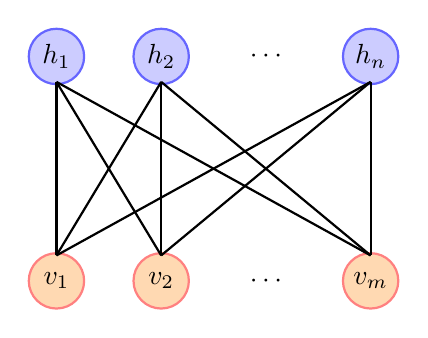
\begin{tikzpicture}[scale=1.9]
			    % \draw ;
			    \node (v1)[neuronv] at (0, 0) {$v_1$};
			    \node (v2)[neuronv] at (0.7, 0) {$v_2$};
			    \node (v3)[] at (1.4, 0) {$\cdots$};
			    \node (v4)[neuronv] at (2.1, 0) {$v_m$};

			    \node (h1)[neuronh] at (0, 1.5) {$h_1$};
			    \node (h2)[neuronh] at (0.7, 1.5) {$h_2$};
			    \node (h3)[] at (1.4, 1.5) {$\cdots$};
			    \node (h4)[neuronh] at (2.1, 1.5) {$h_n$};


			    \onslide<3->{\draw[stateTransition] (0,0.17) -- (0,1.33) node [midway,above=-0.06cm,sloped] {};
			    \draw[stateTransition] (0,0.17) -- (0.7,1.33) node [midway,above=-0.06cm,sloped] {};
			    \draw[stateTransition] (0,0.17) -- (2.1,1.33) node [midway,above=-0.06cm,sloped] {};

			    \draw[stateTransition] (0.7,0.17) -- (0,1.33) node [midway,above=-0.06cm,sloped] {};
			    \draw[stateTransition] (0.7,0.17) -- (0.7,1.33) node [midway,above=-0.06cm,sloped] {};
			    \draw[stateTransition] (0.7,0.17) -- (2.1,1.33) node [midway,above=-0.06cm,sloped] {};

			    \draw[stateTransition] (2.1,0.17) -- (0,1.33) node [midway,above=-0.06cm,sloped] {};
			    \draw[stateTransition] (2.1,0.17) -- (0.7,1.33) node [midway,above=-0.06cm,sloped] {};
			    \draw[stateTransition] (2.1,0.17) -- (2.1,1.33) node [midway,above=-0.06cm,sloped] {};}

			\end{tikzpicture}}

		\end{overlayarea}
		
		\column{0.6\textwidth}
		\begin{overlayarea}{\textwidth}{\textheight}
			\begin{itemize}\justifying
				\item<1-> We return back to our Markov Network containing hidden variables and visible variables
				\item<2-> We will get rid of the image and just keep the hidden and latent variables
				\item<3-> We have edges between each pair of (hidden, visible) variables.
				\item<4-> We do not have edges between (hidden, hidden) and (visible, visible) variables
			\end{itemize}
		\end{overlayarea}
	\end{columns}
\end{frame}

\begin{frame}
	\begin{columns}
		\column{0.4\textwidth}
		\begin{overlayarea}{\textwidth}{\textheight}
			\centering
\vspace{0.5cm}
\tikzstyle{neuronv}=[circle,minimum size=20pt,inner sep=0pt, thick, fill=orange!30, draw=red!50]
\tikzstyle{neuronh}=[circle,minimum size=20pt,inner sep=0pt, thick, fill=blue!20, draw=blue!60]
\tikzstyle{stateTransition}=[thick]
\tikzstyle{learned}=[text=black]
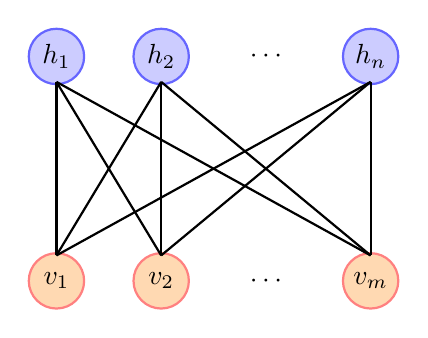
\begin{tikzpicture}[scale=1.9]
    % \draw ;
    \node (v1)[neuronv] at (0, 0) {$v_1$};
    \node (v2)[neuronv] at (0.7, 0) {$v_2$};
    \node (v3)[] at (1.4, 0) {$\cdots$};
    \node (v4)[neuronv] at (2.1, 0) {$v_m$};

    \node (h1)[neuronh] at (0, 1.5) {$h_1$};
    \node (h2)[neuronh] at (0.7, 1.5) {$h_2$};
    \node (h3)[] at (1.4, 1.5) {$\cdots$};
    \node (h4)[neuronh] at (2.1, 1.5) {$h_n$};

	\draw[stateTransition] (0,0.17) -- (0,1.33) node [midway,above=-0.06cm,sloped] {};
    \draw[stateTransition] (0,0.17) -- (0.7,1.33) node [midway,above=-0.06cm,sloped] {};
    \draw[stateTransition] (0,0.17) -- (2.1,1.33) node [midway,above=-0.06cm,sloped] {};

    \draw[stateTransition] (0.7,0.17) -- (0,1.33) node [midway,above=-0.06cm,sloped] {};
    \draw[stateTransition] (0.7,0.17) -- (0.7,1.33) node [midway,above=-0.06cm,sloped] {};
    \draw[stateTransition] (0.7,0.17) -- (2.1,1.33) node [midway,above=-0.06cm,sloped] {};

    \draw[stateTransition] (2.1,0.17) -- (0,1.33) node [midway,above=-0.06cm,sloped] {};
    \draw[stateTransition] (2.1,0.17) -- (0.7,1.33) node [midway,above=-0.06cm,sloped] {};
    \draw[stateTransition] (2.1,0.17) -- (2.1,1.33) node [midway,above=-0.06cm,sloped] {};

\end{tikzpicture}
		\end{overlayarea}
		\column{0.6\textwidth}
		\begin{overlayarea}{\textwidth}{\textheight}
			\begin{itemize}\justifying
				\item<1-> Earlier, we saw that given such a Markov network the joint probability distribution can be written as a product of factors
				\item<2-> Can you tell how many factors are there in this case? 
				\item<3-> Recall that factors correspond to maximal cliques
				\item<4-> What are the maximal cliques in this case? \onslide<5->{every pair of visible and hidden node forms a clique}
				\item<6-> How many such cliques do we have? $(m \times n)$
			\end{itemize}
		\end{overlayarea}
	\end{columns}
\end{frame}

\begin{frame}
	\begin{columns}
		\column{0.4\textwidth}
		\begin{overlayarea}{\textwidth}{\textheight}
			\centering
\vspace{0.5cm}
\tikzstyle{neuronv}=[circle,minimum size=20pt,inner sep=0pt, thick, fill=orange!30, draw=red!50]
\tikzstyle{neuronh}=[circle,minimum size=20pt,inner sep=0pt, thick, fill=blue!20, draw=blue!60]
\tikzstyle{stateTransition}=[thick]
\tikzstyle{learned}=[text=black]
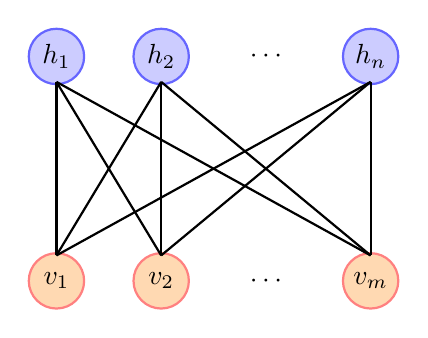
\begin{tikzpicture}[scale=1.9]
    % \draw ;
    \node (v1)[neuronv] at (0, 0) {$v_1$};
    \node (v2)[neuronv] at (0.7, 0) {$v_2$};
    \node (v3)[] at (1.4, 0) {$\cdots$};
    \node (v4)[neuronv] at (2.1, 0) {$v_m$};

    \node (h1)[neuronh] at (0, 1.5) {$h_1$};
    \node (h2)[neuronh] at (0.7, 1.5) {$h_2$};
    \node (h3)[] at (1.4, 1.5) {$\cdots$};
    \node (h4)[neuronh] at (2.1, 1.5) {$h_n$};

	\draw[stateTransition] (0,0.17) -- (0,1.33) node [midway,above=-0.06cm,sloped] {};
    \draw[stateTransition] (0,0.17) -- (0.7,1.33) node [midway,above=-0.06cm,sloped] {};
    \draw[stateTransition] (0,0.17) -- (2.1,1.33) node [midway,above=-0.06cm,sloped] {};

    \draw[stateTransition] (0.7,0.17) -- (0,1.33) node [midway,above=-0.06cm,sloped] {};
    \draw[stateTransition] (0.7,0.17) -- (0.7,1.33) node [midway,above=-0.06cm,sloped] {};
    \draw[stateTransition] (0.7,0.17) -- (2.1,1.33) node [midway,above=-0.06cm,sloped] {};

    \draw[stateTransition] (2.1,0.17) -- (0,1.33) node [midway,above=-0.06cm,sloped] {};
    \draw[stateTransition] (2.1,0.17) -- (0.7,1.33) node [midway,above=-0.06cm,sloped] {};
    \draw[stateTransition] (2.1,0.17) -- (2.1,1.33) node [midway,above=-0.06cm,sloped] {};

\end{tikzpicture}
		\end{overlayarea}
		\column{0.6\textwidth}
		\begin{overlayarea}{\textwidth}{\textheight}
			\footnotesize{
				\begin{itemize}\justifying
					\item<1-> So we can write the joint pdf as a product of the following factors
					\begin{align*}
					P(V, H) = \frac{1}{Z}\prod_i\prod_j \phi_{ij}(v_i, h_j)
					\end{align*}
					\item<2-> In fact, we can also add additional factors corresponding to the nodes and write
					\begin{align*}
					P(V, H) = \frac{1}{Z}\prod_i\prod_j \phi_{ij}(v_i, h_j) \prod_i \psi_i(v_i) \prod_j \xi_j(h_j) 
					\end{align*}
					\item<3-> It is legal to do this (i.e., add factors for $\psi_i(v_i) \xi_j(h_j))$ as long as we ensure that $Z$ is adjusted in a way that the resulting quantity is a probability distribution
					\item<4-> $Z$ is the partition function and is given by
					\begin{align*}
					\sum_V \sum_H \prod_i\prod_j \phi_{ij}(v_i, h_j) \prod_i \psi_i(v_i) \prod_j \xi_j(h_j)
					\end{align*}
				\end{itemize}
			}
		\end{overlayarea}
	\end{columns}
\end{frame}

\begin{frame}
	\begin{columns}
		\column{0.4\textwidth}
		\begin{overlayarea}{\textwidth}{\textheight}
			\centering
\vspace{0.5cm}
\tikzstyle{neuronv}=[circle,minimum size=20pt,inner sep=0pt, thick, fill=orange!30, draw=red!50]
\tikzstyle{neuronh}=[circle,minimum size=20pt,inner sep=0pt, thick, fill=blue!20, draw=blue!60]
\tikzstyle{stateTransition}=[thick]
\tikzstyle{learned}=[text=black]
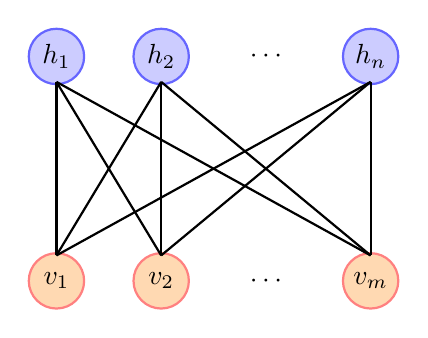
\begin{tikzpicture}[scale=1.9]
    % \draw ;
    \node (v1)[neuronv] at (0, 0) {$v_1$};
    \node (v2)[neuronv] at (0.7, 0) {$v_2$};
    \node (v3)[] at (1.4, 0) {$\cdots$};
    \node (v4)[neuronv] at (2.1, 0) {$v_m$};

    \node (h1)[neuronh] at (0, 1.5) {$h_1$};
    \node (h2)[neuronh] at (0.7, 1.5) {$h_2$};
    \node (h3)[] at (1.4, 1.5) {$\cdots$};
    \node (h4)[neuronh] at (2.1, 1.5) {$h_n$};

	\draw[stateTransition] (0,0.17) -- (0,1.33) node [midway,above=-0.06cm,sloped] {};
    \draw[stateTransition] (0,0.17) -- (0.7,1.33) node [midway,above=-0.06cm,sloped] {};
    \draw[stateTransition] (0,0.17) -- (2.1,1.33) node [midway,above=-0.06cm,sloped] {};

    \draw[stateTransition] (0.7,0.17) -- (0,1.33) node [midway,above=-0.06cm,sloped] {};
    \draw[stateTransition] (0.7,0.17) -- (0.7,1.33) node [midway,above=-0.06cm,sloped] {};
    \draw[stateTransition] (0.7,0.17) -- (2.1,1.33) node [midway,above=-0.06cm,sloped] {};

    \draw[stateTransition] (2.1,0.17) -- (0,1.33) node [midway,above=-0.06cm,sloped] {};
    \draw[stateTransition] (2.1,0.17) -- (0.7,1.33) node [midway,above=-0.06cm,sloped] {};
    \draw[stateTransition] (2.1,0.17) -- (2.1,1.33) node [midway,above=-0.06cm,sloped] {};

\end{tikzpicture}
			\begin{center}
				\begin{table}
				\only<3->{\scalebox{0.6}{
					\begin{tabular}{|ccp{1cm}|}
						\hline
						\multicolumn{3}{|c|}{$\phi_{11}(v_1,h_1)$} \\ \hline
						$0$       & $0$       & 30\\
						$0$       & $1$       & 5 \\
						$1$       & $0$       & 1 \\
						$1$       & $1$       & 10\\ \hline
					\end{tabular}}}
				\end{table}
				\begin{table}
				\only<5->{\scalebox{0.6}{
					\begin{tabular}{|cp{1cm}|}
						\hline
						\multicolumn{2}{|c|}{$\psi_{1}(v_1)$} \\ \hline
						$0$        & 10\\
						$1$        & 2 \\ \hline
					\end{tabular}}}
				\end{table}
			\end{center}
		\end{overlayarea}
		\column{0.6\textwidth}
		\begin{overlayarea}{\textwidth}{\textheight}
			\begin{itemize}\justifying

				\item<1-> Let us understand each of these factors in more detail
				\item<2-> For example, $\phi_{11}(v_1, h_1)$ is a factor which takes the values of $v_1 \in \{0, 1\}$ and $h_1 \in \{0, 1\}$ and returns a value indicating the affinity between these two variables
				\item<3-> The adjoining table shows one such possible instantiation of the $\phi_{11}$ function
				\item<4-> Similarly, $\psi_1(v_1)$ takes the value of $v_1 \in \{0, 1\}$ and gives us a number which roughly indicates the possibility of $v_1$ taking on the value 1 or 0
				\item<5-> The adjoining table shows one such possible instantiation of the $\psi_{11}$ function
				\item<6-> A similar interpretation can be made for $\xi_1(h_1)$
			\end{itemize}
		\end{overlayarea}
	\end{columns}
\end{frame}


\begin{frame}
	\begin{block}{}
		Just to be sure that we understand this correctly let us take a small example where $|V| = 3$ (i.e., $V \in \{0,1\}^3$) and $|H| = 2$ (i.e., $H \in \{0,1\}^2$)
	\end{block}
\end{frame}


\begin{frame}
	\begin{columns}
		\column{0.4\textwidth}
		\begin{overlayarea}{\textwidth}{\textheight}
			\centering
			\vspace{0.5cm}
			\tikzstyle{neuronv}=[circle,minimum size=20pt,inner sep=0pt, thick, fill=orange!30, draw=red!50]
			\tikzstyle{neuronh}=[circle,minimum size=20pt,inner sep=0pt, thick, fill=blue!30, draw=blue!60]
			\tikzstyle{stateTransition}=[thick]
			\tikzstyle{learned}=[text=black]
			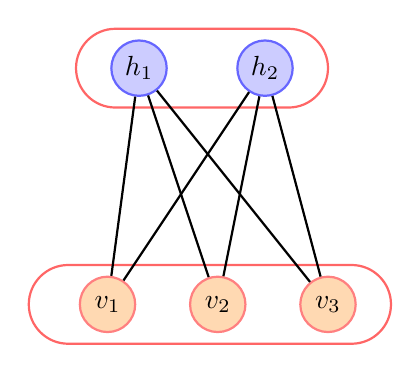
\begin{tikzpicture}[scale=2]
			    % \draw ;
			    \draw[rounded corners=0.5cm, draw=red!60, thick] (-0.5, -0.25) rectangle (1.8, 0.25) {};
			    \draw[rounded corners=0.5cm, draw=red!60, thick] (-0.2, 1.25) rectangle (1.4, 1.75) {};

			    \node (v1)[neuronv] at (0, 0) {$v_1$};
			    \node (v2)[neuronv] at (0.7, 0) {$v_2$};
			    \node (v3)[neuronv] at (1.4, 0) {$v_3$};
			    % \node[below=0.5cm of v2] (v) {$\textbf{v} \in \{0, 1\}^m$};
			    % \node[learned,below=0.1cm of v1] (bv1) {$b_1$};
			    % \node[learned,below=0.1cm of v2] (bv2) {$b_2$};
			    % \node[learned,below=0.1cm of v3, scale=0.7] (bv3) {$b_1$};
			    % \node[learned,below=0.1cm of v4] (bv4) {$b_m$};

			    \node (h1)[neuronh] at (0.2, 1.5) {$h_1$};
			    \node (h2)[neuronh] at (1.0, 1.5) {$h_2$};
			    % \node[above=0.5cm of h2] (h) {$\textbf{h} \in \{0, 1\}^n$};
			    % \node[learned,above=0.1cm of h1] (bv1) {$c_1$};
			    % \node[learned,above=0.1cm of h2] (bv2) {$c_2$};
			    % \node[learned,below=0.1cm of v3, scale=0.7] (bv3) {$b_{v_3}$};
			    % \node[learned,above=0.1cm of h4] (bv4) {$c_n$};

			    % \node[learned, scale=0.7] (W) at (2.5, 0.5) {$W \in \mathbb{R}^{m \times n}$};

			    \draw[learned,stateTransition] (v1) -- (h1) node [midway,left=-0.1cm] {};
			    \draw[stateTransition] (v1) -- (h2) node [midway,above=-0.06cm,sloped] {};

			    \draw[stateTransition] (v2) -- (h1) node [midway,above=-0.06cm,sloped] {};
			    \draw[stateTransition] (v2) -- (h2) node [midway,above=-0.06cm,sloped] {};

			    \draw[stateTransition] (v3) -- (h1) node [midway,above=-0.06cm,sloped] {};
			    \draw[stateTransition] (v3) -- (h2) node [midway,above=-0.06cm,sloped] {};

			\end{tikzpicture}
			\begin{center}
			\begin{table}
				\scalebox{0.4}{
				\begin{tabular}{|ccc|ccc|ccc|ccc|ccc|ccc|}
				\hline
				\multicolumn{3}{|c|}{$\phi_{11}(v_1,h_1)$} & \multicolumn{3}{c|}{$\phi_{12}(v_1,h_2)$} & \multicolumn{3}{c|}{$\phi_{21}(v_2,h_1)$} & \multicolumn{3}{c|}{$\phi_{22}(v_2,h_2)$} & \multicolumn{3}{|c|}{$\phi_{31}(v_3,h_1)$} & \multicolumn{3}{c|}{$\phi_{32}(v_3,h_2)$}\\ \hline
				$0$        & $0$       & 20       & $0$        & $0$       & 6       & $0$       & $0$       & 3       & $0$       & $0$       & 2       & $0$        & $0$       & 6       & $0$       & $0$       & 3 \\
				$0$        & $1$       & 3       & $0$        & $1$       & 20       & $0$       & $1$       & 3       & $0$       & $1$       & 1      & $0$       & $1$       & 3       & $0$       & $1$       & 1  \\
				$1$        & $0$       & 5       & $1$        & $0$       & 10       & $1$       & $0$       & 2       & $1$       & $0$       & 10      & $1$        & $0$       & 5       & $1$        & $0$       & 10\\
				$1$        & $1$       & 10       & $1$        & $1$       & 2       & $1$       & $1$       & 10       & $1$       & $1$       & 10      & $1$       & $1$       & 10       & $1$       & $1$       & 10 \\ \hline
				\end{tabular}}
					\scalebox{0.4}{
				\begin{tabular}{|cc|cc|cc|cc|cc|}
				\hline
				\multicolumn{2}{|c|}{$\psi_{1}(v_1)$} & \multicolumn{2}{c|}{$\psi_{2}(v_2)$} & \multicolumn{2}{c|}{$\psi_{3}(v_3)$} &\multicolumn{2}{c|}{$\xi_{1}(h_1)$} & \multicolumn{2}{c|}{$\xi_{2}(h_2)$}\\ \hline
				$0$      & 30      & $0$      & 100      & $0$       & 1        & $0$      & 100 & $0$      & 10      \\
				$1$       & 1       & $1$      & 1        & $1$      & 100      & $1$      & 1   & $1$      & 10     \\ \hline
				\end{tabular}}
			\end{table}
			\end{center}
		\end{overlayarea}
		\column{0.6\textwidth}
		\begin{overlayarea}{\textwidth}{\textheight}
			\begin{itemize}\justifying
				\item<1-> Suppose we are now interested in $P(V=<0,0,0>, H=<1,1>)$ 
				\item<2-> We can compute this using the following function
				\begin{align*}
				P(V&=<0,0,0>, H=<1,1>) \\
				= &\frac{1}{Z}\phi_{11}(0, 1) \phi_{12}(0,1) \phi_{21}(0,1)\\
				&\phi_{22}(0,1)\phi_{31}(0,1)\phi_{32}(0,1)\\
				&\psi_1(0) \psi_2(0) \psi_3(0)  \xi_1(1) \xi_2(1) 
				\end{align*}
				\item<3-> and the partition function will be given by
				\begin{align*}
					\sum_{v_1 = 0}^1 & \sum_{v_2 = 0}^1 \sum_{v_3 = 0}^1\sum_{h_1 = 0}^1 \sum_{h_2 = 1}^1  \\
					&P(V=<v_1,v_2,v_3>, H=<h_1,h_2>) 
				\end{align*}
			\end{itemize}
		\end{overlayarea}
	\end{columns}
\end{frame}


\begin{frame}
	\begin{columns}
		\column{0.4\textwidth}
		\begin{overlayarea}{\textwidth}{\textheight}
			\centering
			\vspace{0.5cm}
			\tikzstyle{neuronv}=[circle,minimum size=20pt,inner sep=0pt, thick, fill=orange!30, draw=red!50]
			\tikzstyle{neuronh}=[circle,minimum size=20pt,inner sep=0pt, thick, fill=blue!20, draw=blue!60]
			\tikzstyle{stateTransition}=[thick]
			\tikzstyle{learned}=[text=black]
			\begin{tikzpicture}[scale=1.9]
			    % \draw ;
			    \onslide<4->{\draw[rounded corners=0.5cm, draw=red!60, thick] (-0.4, -0.25) rectangle (2.5, 0.25) {};
			    \draw[rounded corners=0.5cm, draw=red!60, thick] (-0.4, 1.25) rectangle (2.5, 1.75) {};}

			    \node (v1)[neuronv] at (0, 0) {$v_1$};
			    \node (v2)[neuronv] at (0.7, 0) {$v_2$};
			    \node (v3)[] at (1.4, 0) {$\cdots$};
			    \node (v4)[neuronv] at (2.1, 0) {$v_m$};
			    \onslide<4->{\node[below=0.5cm of v2] (v) {$V \in \{0, 1\}^m$};
			    \node[learned,below=0.1cm of v1] (bv1) {$b_1$};
			    \node[learned,below=0.1cm of v2] (bv2) {$b_2$};
			    % \node[learned,below=0.1cm of v3, scale=0.7] (bv3) {$b_{v_3}$};
			    \node[learned,below=0.1cm of v4] (bv4) {$b_m$};}

			    \node (h1)[neuronh] at (0, 1.5) {$h_1$};
			    \node (h2)[neuronh] at (0.7, 1.5) {$h_2$};
			    \node (h3)[] at (1.4, 1.5) {$\cdots$};
			    \node (h4)[neuronh] at (2.1, 1.5) {$h_n$};
			    \onslide<4->{\node[above=0.5cm of h2] (h) {$H \in \{0, 1\}^n$};
			    \node[learned,above=0.1cm of h1] (bv1) {$c_1$};
			    \node[learned,above=0.1cm of h2] (bv2) {$c_2$};
			    % \node[learned,below=0.1cm of v3, scale=0.7] (bv3) {$b_{v_3}$};
			    \node[learned,above=0.1cm of h4] (bv4) {$c_n$};

			    \node[learned, scale=0.7] (W) at (2.5, 0.75) {$W \in \mathbb{R}^{m \times n}$};}

			    \only<1-3>{\draw[learned,stateTransition] (0,0.17) -- (0,1.33) node [midway,left=-0.1cm] {};}
			    \only<4->{\draw[learned,stateTransition] (0,0.17) -- (0,1.33) node [midway,left=-0.1cm] {$w_{1,1}$};}
			    \draw[stateTransition] (0,0.17) -- (0.7,1.33) node [midway,above=-0.06cm,sloped] {};
			    \draw[stateTransition] (0,0.17) -- (2.1,1.33) node [midway,above=-0.06cm,sloped] {};

			    \draw[stateTransition] (0.7,0.17) -- (0,1.33) node [midway,above=-0.06cm,sloped] {};
			    \draw[stateTransition] (0.7,0.17) -- (0.7,1.33) node [midway,above=-0.06cm,sloped] {};
			    \draw[stateTransition] (0.7,0.17) -- (2.1,1.33) node [midway,above=-0.06cm,sloped] {};

			    \draw[stateTransition] (2.1,0.17) -- (0,1.33) node [midway,above=-0.06cm,sloped] {};
			    \draw[stateTransition] (2.1,0.17) -- (0.7,1.33) node [midway,above=-0.06cm,sloped] {};
			    \only<1-3>{\draw[learned,stateTransition] (2.1,0.17) -- (2.1,1.33) node [midway,left=-0.1cm] {};}
			    \only<4->{\draw[learned,stateTransition] (2.1,0.17) -- (2.1,1.33) node [midway,left=-0.1cm] {$w_{m,n}$};}
			\end{tikzpicture}
		\end{overlayarea}
		\column{0.6\textwidth}
		\begin{overlayarea}{\textwidth}{\textheight}
			\begin{itemize}\justifying
				\item<1-> How do we learn these clique potentials: $\phi_{ij}(v_i, h_j), \psi_i(v_i), \xi_j(h_j)$?
				\item<2->  Whenever we want to learn something what do we introduce? \onslide<3->{(parameters)}
				\item<4-> So we will introduce a parametric form for these clique potentials and then learn these parameters
				\item<5-> The specific parametric form chosen by RBMs is 
				\begin{align*}
					&\phi_{ij}(v_i, h_j) = e^{w_{ij} v_i h_j}\\
					&\psi_i(v_i) = e^{b_i v_i}\\
					&\xi_j(h_j) = e^{c_j h_j}\\
				\end{align*}
			\end{itemize}
		\end{overlayarea}
	\end{columns}
\end{frame}


\begin{frame}
	\begin{columns}
		\column{0.4\textwidth}
		\begin{overlayarea}{\textwidth}{\textheight}
			\input{modules/Module3/tikz_images/rbm}
		\end{overlayarea}
		\column{0.6\textwidth}
		\begin{overlayarea}{\textwidth}{\textheight}
			\begin{itemize}\justifying
				\item<1-> With this parametric form, let us see what the joint distribution looks like
				\begin{align*}
					\onslide<2->{&P(V, H) = \frac{1}{Z}\prod_i\prod_j \phi_{ij}(v_i, h_j) \prod_i \psi_i(v_i) \prod_j \xi_j(h_j)\\}
					\onslide<3->{&= \frac{1}{Z}\prod_i\prod_j e^{w_{ij} v_i h_j} \prod_i e^{b_i v_i} \prod_j e^{c_j h_j}\\}
					\onslide<4->{&= \frac{1}{Z} e^{\sum_i\sum_j w_{ij} v_i h_j}  e^{\sum_i b_i v_i} e^{\sum_j c_j h_j}\\}
					\onslide<5->{&= \frac{1}{Z} e^{\sum_i\sum_j w_{ij} v_i h_j  +\sum_i b_i v_i +\sum_j c_j h_j}\\}
					\onslide<6->{&= \frac{1}{Z} e^{-E(V,H)} \text{  where,}\\}
					\onslide<7->{& E(V,H) = -\sum_i\sum_j w_{ij} v_i h_j  -\sum_i b_i v_i -\sum_j c_j h_j}
				\end{align*} 
			\end{itemize}
		\end{overlayarea}
	\end{columns}
\end{frame}


\begin{frame}
	\begin{columns}
		\column{0.4\textwidth}
		\begin{overlayarea}{\textwidth}{\textheight}
			\input{modules/Module3/tikz_images/rbm}
		\end{overlayarea}
		\column{0.6\textwidth}
		\begin{overlayarea}{\textwidth}{\textheight}
			\begin{align*}
				E(V,H) = -\sum_i\sum_j w_{ij} v_i h_j  -\sum_i b_i v_i -\sum_j c_j h_j
			\end{align*} 
			\begin{itemize}\justifying
				\item<1-> Because of the above form, we refer to these networks as (restricted) Boltzmann machines
				\item<2-> The term comes from statistical mechanics where the distribution of particles in a system over various possible states is given by
				\begin{align*}
					F(state) \propto e^{-\frac{E}{kt}}
				\end{align*}
				\item[]<3-> which is called the Boltzmann distribution or the Gibbs distribution
			\end{itemize}
		\end{overlayarea}
	\end{columns}
\end{frame}
